\documentclass[a4paper,12pt]{article} % добавить leqno в [] для нумерации слева
\usepackage[a4paper,top=1.3cm,bottom=2cm,left=1.5cm,right=1.5cm,marginparwidth=0.75cm]{geometry}
%%% Работа с русским языком
\usepackage{cmap}					% поиск в PDF
\usepackage{mathtext} 				% русские буквы в фомулах
\usepackage[T2A]{fontenc}			% кодировка
\usepackage[utf8]{inputenc}			% кодировка исходного текста
\usepackage[english,russian]{babel}	% локализация и переносы
\usepackage{multirow}

\usepackage{graphicx}

\usepackage{wrapfig}
\usepackage{tabularx}

\usepackage{hyperref}
\usepackage[rgb]{xcolor}
\hypersetup{
colorlinks=true,urlcolor=blue
}

%%% Дополнительная работа с математикой
\usepackage{amsmath,amsfonts,amssymb,amsthm,mathtools} % AMS
\usepackage{icomma} % "Умная" запятая: $0,2$ --- число, $0, 2$ --- перечисление

%% Номера формул
\mathtoolsset{showonlyrefs=true} % Показывать номера только у тех формул, на которые есть \eqref{} в тексте.

%% Шрифты
\usepackage{euscript}	 % Шрифт Евклид
\usepackage{mathrsfs} % Красивый матшрифт

%% Свои команды
\DeclareMathOperator{\sgn}{\mathop{sgn}}

%% Перенос знаков в формулах (по Львовскому)
\newcommand*{\hm}[1]{#1\nobreak\discretionary{}
{\hbox{$\mathsurround=0pt #1$}}{}}

%% Графики
\usepackage{tikz}
\usepackage{pgfplots}
\pgfplotsset{compat=1.9}

\date{\today}

\begin{document}

\begin{titlepage}
	\begin{center}
		{\large МОСКОВСКИЙ ФИЗИКО-ТЕХНИЧЕСКИЙ ИНСТИТУТ (НАЦИОНАЛЬНЫЙ ИССЛЕДОВАТЕЛЬСКИЙ УНИВЕРСИТЕТ)}
	\end{center}
	\begin{center}
		{\large Физтех-школа аэрокосмических технологий}
	\end{center}
	
	
	\vspace{4.5cm}
	{\huge
		\begin{center}
			{\bf Отчёт о выполнении лабораторной работы 2.4.1}\\
			Определение теплоты испарения жидкости
		\end{center}
	}
	\vspace{1cm}
	\begin{center}
		{\large Соболевский Федор Александрович \\
			\vspace{0.2cm}
			Б03-109}
	\end{center}
	\vspace{8cm}
	\begin{center}
		Апрель 2022
	\end{center}
\end{titlepage}

\section{Аннотация}

В данной температуре исследована зависимость давления насыщенных паров воды от её температуры. Полученные значения применены для вычисления молярной и удельной теплоты испарения воды. Проанализированы методы измерения давления насыщенных паров и их погрешности.

\section{Теоретические сведения}

\subsection{Вычисление теплоты испарения}

Количество теплоты, необходимое для изотермического испарения одного моля жидкости при внешнем давлении, равном упругости ее насыщенных паров, называется молярной теплотой испарения (парообразования). В данной работе применён метод, основанный на уравнении Клапейрона-Клаузиуса:

\begin{equation}
    \frac{dP}{dT} = \frac{L}{T(V_2 - V_1)},
    \label{ClapeyronClausius}
\end{equation}

где $T$ - абсолютная температура, $P$ - давление насыщенного пара при данной температуре, $L$ - теплота испарения жидкости, $V_2$ - объём пара, $V_1$ - объём жидкости. 

В используемом приборе измерения проводятся при давлениях значительно ниже атмосферного, что позволяет сделать ряд упрощений. Во-первых, молярный объём воды составляет не более 0,2\% от молярного объёма пара, что заметно меньше погрешности измерений, поэтому при расчётах величиной $V_1$ можно пренебречь. Во-вторых, величины $a/V^2$ и $b$, возникающие при описании водяного пара уравнением газа Ван-дер-Ваальса, также достаточно малы по сравнению с измеряемыми величинами, чтобы можно было применить уравнение Клапейрона, откуда

\begin{equation}
    V = \frac{RT}{P}.
    \label{volume}
\end{equation}

Подставляя \eqref{volume} в \eqref{ClapeyronClausius} и пренебрегая $V_1$, получаем выражение для теплоты испарения:

\begin{equation}
    L = \frac{RT^2}{P}\frac{dP}{dT} = -R\frac{d(\ln P)}{d(1/T)}.
    \label{finalEq}
\end{equation}

Удельную теплоту испарения можно найти как 

\begin{equation}
    \lambda = L/\mu.
    \label{final2}
\end{equation}

\subsection{Экспериментальная установка}

\begin{figure}
    \centering
    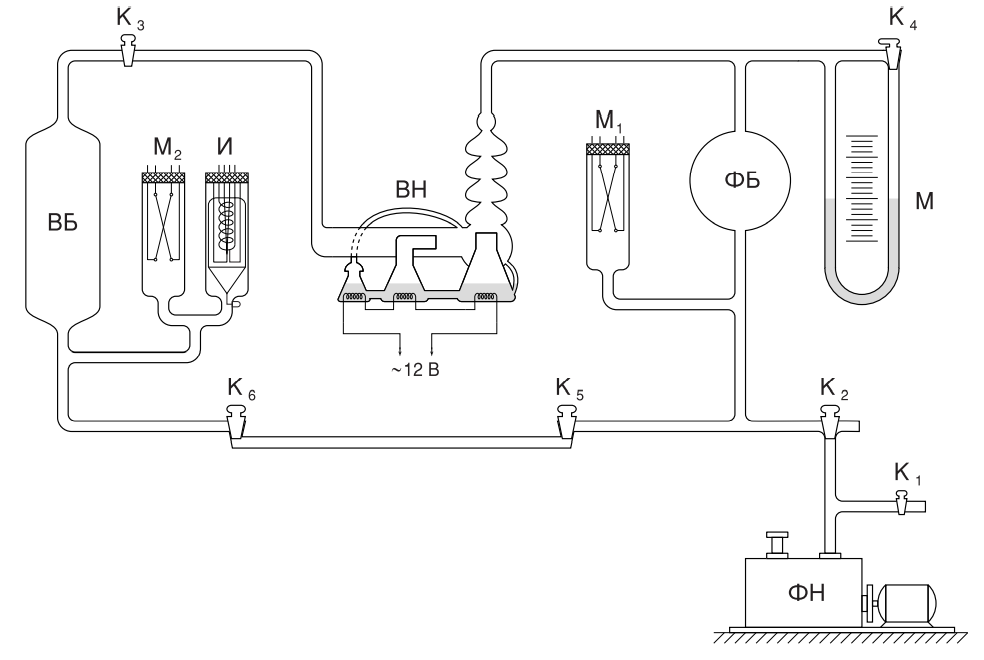
\includegraphics[width = 0.8\textwidth]{setup.PNG}
    \caption{Схема экспериментальной установки}
    \label{fig:setup}
\end{figure}

На рисунке приведена схема установки с использованием современного термостата. Установка включает термостат A, экспериментальный прибор B и отсчетный микроскоп C. Экспериментальный прибор B представляет собой емкость 12, заполненную водой. В нее погружен запаянный прибор 13 с исследуемой жидкостью 14. Перед заполнением исследуемой жидкости воздух из запаянного прибора был удален, так что над жидкостью находится только её насыщенный пар. Давление пара определяется по ртутному манометру 15, соединенному с емкостью 13. Численная величина давления измеряется по разности показаний отсчетного микроскопа 16, настраиваемого последовательно на нижний и верхний уровни столбика ртути манометра. Показания микроскопа снимаются по шкале 17.

\section{Оборудование и инструментальные погрешности}

\textbf{В работе использовались:} термостат, герметичный сосуд с исследуемой жидкостью (водой), отсчётный микроскоп, штангенциркуль.

\textbf{Инструментальные погрешности:} 

\begin{itemize}
    \item \textbf{Штангенциркуль:} $\Delta_h = 0,1$ мм;
    \item \textbf{Термометр термостата:} $\Delta_T = 0,1$ К.
\end{itemize}

\section{Результаты измерений и обработка экспериментальных данных}

Перепад давлений в установке измерялся по разности высот колен ртутного манометра. Величину давления насыщенных паров $P_0$ можно определить по формуле $P_0 = \rho g\Delta H$, где плотность ртути $\rho = 13600$ кг/м$^3$. Также было необходимо учесть ошибку, связанную с возникновением в правом колене прибора столбика воды высотой 4,2 мм, что даёт ошибку $\Delta P = (1000 - 13600) \cdot 0,0042 \cdot 9,81 = -519,14$ (Па). 

Результаты измерения давления насыщенных паров при разных температурах при нагревании и охлаждении представлены в таблицах \ref{tab:heating} и \ref{tab:cooling} соответственно. Графики зависимости давления насыщенного пара от температуры в каждом опыте представлены на рисунках \ref{graph:heating} и \ref{graph:cooling}. 

\begin{table}[]
    \centering
    \begin{tabular}{|c|c|c|c|c|c|c|}\hline
        $t$, $^\text{o}$C & $T$, К & $\Delta h$, мм & $P_0$, кПа & $P$, кПа & $1/T$, 10$^{-3}$ К$^{-1}$ & $\ln P$ \\ \hline
        23 & 296,15 & 19,1 & 2,55 & 2,03 & 3,377 & 7,62 \\ \hline
        24 & 297,15 & 20,5 & 2,74 & 2,22 & 3,365 & 7,70 \\ \hline
        25 & 298,15 & 21,9 & 2,92 & 2,40 & 3,354 & 7,78 \\ \hline
        26 & 299,15 & 23,5 & 3,14 & 2,62 & 3,343 & 7,87 \\ \hline
        27 & 300,15 & 24,9 & 3,32 & 2,80 & 3,332 & 7,94 \\ \hline
        28 & 301,15 & 26,3 & 3,51 & 2,99 & 3,321 & 8,00 \\ \hline
        29 & 302,15 & 28,5 & 3,80 & 3,28 & 3,310 & 8,10 \\ \hline
        30 & 303,15 & 29,5 & 3,94 & 3,42 & 3,299 & 8,14 \\ \hline
        31 & 304,15 & 31,2 & 4,16 & 3,64 & 3,288 & 8,20 \\ \hline
        32 & 305,15 & 33,4 & 4,46 & 3,94 & 3,277 & 8,28 \\ \hline
        33 & 306,15 & 35,4 & 4,75 & 4,23 & 3,266 & 8,35 \\ \hline
        34 & 307,15 & 37,6 & 5,02 & 4,50 & 3,256 & 8,41 \\ \hline
        35 & 308,15 & 39,8 & 5,31 & 4,79 & 3,245 & 8,47 \\ \hline
        36 & 309,15 & 42,6 & 5,68 & 5,16 & 3,235 & 8,55 \\ \hline
        37 & 310,15 & 44,4 & 5,92 & 5,41 & 3,224 & 8,59 \\ \hline
        \end{tabular}
    \caption{Зависимость давления насыщенного пара от температуры при нагревании}
    \label{tab:heating}
\end{table}

\begin{figure}
\centering
\resizebox {0.55\textwidth} {!} {
\begin{tikzpicture}
\begin{axis}[ xlabel = {$1/T$, 10$^{-3}$ К$^{-1}$}, ylabel = {$\ln P$}, xmin = 3.22, xmax = 3.38, ymin = 7.59, ymax = 8.61, legend style={legend style={at={(axis cs:3.38, 8.61)},anchor=north east}}]
\addplot[color=black, mark=x, only marks] coordinates{
(3.377, 7.62)
(3.365, 7.7)
(3.354, 7.78)
(3.343, 7.87)
(3.332, 7.94)
(3.321, 8)
(3.31, 8.1)
(3.299, 8.14)
(3.288, 8.2)
(3.277, 8.28)
(3.266, 8.35)
(3.256, 8.41)
(3.245, 8.47)
(3.235, 8.55)
(3.224, 8.59)};
\addplot[color=blue] coordinates{(3.225, 8.61)(3.38, 7.6)};
\end{axis}
\end{tikzpicture}
}
\caption{График зависимости давления насыщенного пара от температуры при нагревании}
\label{graph:heating}
\end{figure}

\begin{table}[]
    \centering
    \begin{tabular}{|c|c|c|c|c|c|c|}\hline
        $t$, $^\text{o}$C & $T$, К & $\Delta h$, мм & $P_0$, кПа & $P$, кПа & $1/T$, 10$^{-3}$ К$^{-1}$ & $\ln P$ \\ \hline
        36 & 309,15 & 43,4 & 5,79 & 5,27 & 3,235 & 8,57 \\ \hline
        35 & 308,15 & 40,8 & 5,44 & 4,92 & 3,245 & 8,50 \\ \hline
        34 & 307,15 & 39,0 & 5,20 & 4,68 & 3,256 & 8,45 \\ \hline
        33 & 306,15 & 37,4 & 4,99 & 4,47 & 3,266 & 8,41 \\ \hline
        32 & 305,15 & 35,0 & 4,67 & 4,15 & 3,277 & 8,33 \\ \hline
        31 & 304,15 & 33,2 & 4,43 & 3,91 & 3,288 & 8,27 \\ \hline
        30 & 303,15 & 31,2 & 4,16 & 3,64 & 3,299 & 8,20 \\ \hline
        29 & 302,15 & 28,4 & 3,79 & 3,27 & 3,310 & 8,09 \\ \hline
        28 & 301,15 & 25,2 & 3,36 & 2,84 & 3,321 & 7,95 \\ \hline
        26 & 299,15 & 22,0 & 2,94 & 2,42 & 3,343 & 7,79 \\ \hline
    \end{tabular}
    \caption{Зависимость давления насыщенного пара от температуры при охлаждении}
    \label{tab:cooling}
\end{table}

\begin{figure}
\centering
\resizebox {0.55\textwidth} {!} {
\begin{tikzpicture}
\begin{axis}[ xlabel = {$1/T$, 10$^{-3}$ К$^{-1}$}, ylabel = {$\ln P$}, xmin = 3.23, xmax = 3.35, ymin = 7.7, ymax = 8.61, legend style={legend style={at={(axis cs:3.38, 8.61)},anchor=north east}}]
\addplot[color=black, mark=x, only marks] coordinates{
(3.343, 7.79)
(3.321, 7.95)
(3.31, 8.09)
(3.299, 8.2)
(3.288, 8.27)
(3.277, 8.33)
(3.266, 8.41)
(3.256, 8.45)
(3.245, 8.5)
(3.235, 8.57)};
\addplot[color=blue] coordinates{(3.23, 8.6)(3.35, 7.779)};
\end{axis}
\end{tikzpicture}
}
\caption{График зависимости давления насыщенного пара от температуры при охлаждении}
\label{graph:cooling}
\end{figure}

Величину $d(\ln P)/d(1/T)$ и случайную погрешность её определения можно вычислить как коэффициент наклона наилучшей прямой и погрешность его определения соответственно с помощью метода наименьших квадратов:

\begin{equation}
    \frac{d(\ln P)}{d(1/T)} = \frac{\langle \ln{P}\cdot 1/T\rangle-\langle \ln{P}\rangle \langle 1/T\rangle}{\langle (1/T)^2\rangle - \langle 1/T\rangle^2},
\end{equation}

\begin{equation}
    \sigma_\text{случ} = \sqrt{\frac{1}{N}\left(\frac{\langle (\ln{P})^2 \rangle - \langle \ln{P} \rangle^2}{\langle (1/T)^2 \rangle - \langle 1/T \rangle^2} - (\frac{d(\ln P)}{d(1/T)})^2 \right)}.
\end{equation}

Систематическая и полная погрешности измерения $dP/dT$ определяются как

\begin{equation}
    \sigma_\text{сист} = \sqrt{(\frac{\Delta_T}{T})^2 + (\frac{\ln(\rho g\Delta_h)}{\ln P})^2}
\end{equation}

\begin{equation}
    \sigma_\text{полн} = \sqrt{\sigma_\text{случ}^2 + \sigma_\text{сист}^2}.
\end{equation}

Отсюда можно найти значения $L$ и $\lambda$ в каждом опыте. Результаты вычислений представлены в таблице \ref{tab:results}.

\begin{table}[]
    \centering
    \begin{tabular}{|c|c|c|c|}\hline
        № опыта & $d(\ln P)/d(1/T)$, $10^{-3}$ К & $L$, кДж/моль & $\lambda$, МДж/кг \\ \hline
        1 & $-6,38 \pm 0,07$ & $53,0 \pm 0,6$ & $2,95 \pm 0,03$ \\ \hline
        2 & $-7,16 \pm 0,28$ & $59,5 \pm 2,3$ & $3,30 \pm 0,13$ \\ \hline
    \end{tabular}
    \caption{Результаты вычисления теплоты испарения воды}
    \label{tab:results}
\end{table}

\section{Обсуждение результатов и выводы}

В данной работе были получены два значения удельной теплоты парообразования воды:

\begin{enumerate}
    \item $\lambda$ = $2,95 \pm 0,03$ МДж/кг;
    \item $\lambda$ = $3,30 \pm 0,13$ МДж/кг.
\end{enumerate}

Ошибка измерений во втором опыте оказалась в несколько раз больше, чем в первом. Причиной тому могло послужить замедленное остывание исследуемой жидкости и меньшее количество измерений. Вследствие этого конечным результатом измерений будем считать значение, полученное в первом опыте.

Табличное значение удельной теплоты парообразования $\lambda_\text{табл} = 2,26$ МДж/кг. Полученное в эксперименте значение отличается от табличного на 30\%. Повышенное значение теплоты парообразования связано, прежде всего, с неточностью измерений с помощью ртутного манометра. Дефект измерений, возникший из-за образования скоплений воды в ртути, сложно оценить точно из-за поверхностных эффектов на границе раздела жидкостей и наличию более мелких вкраплений воды. Также нельзя достаточно точно оценить неидеальность откачки воздуха из установки и давление паров ртути в коленах. Всё это привело с заниженным результатам измерения давления и, как следствие, значительно завышенному значению теплоты парообразования. 

Однако полученное значение не отличается от табличного по порядку, а зависимость $\ln P$ от $1/T$ действительно близка к линейной в измеряемом диапазоне температур. Это говорит о том, что при наличии более точного оборудования для измерения давления рассмотренный метод применим для измерения теплоты испарения жидкости.

\end{document}